% !TeX spellcheck = en_GB
%%%%%% 20/12 DT
\noindent\begin{minipage}%[t][0.55\textheight]
[t]{.59\textwidth}
  	\centering
  		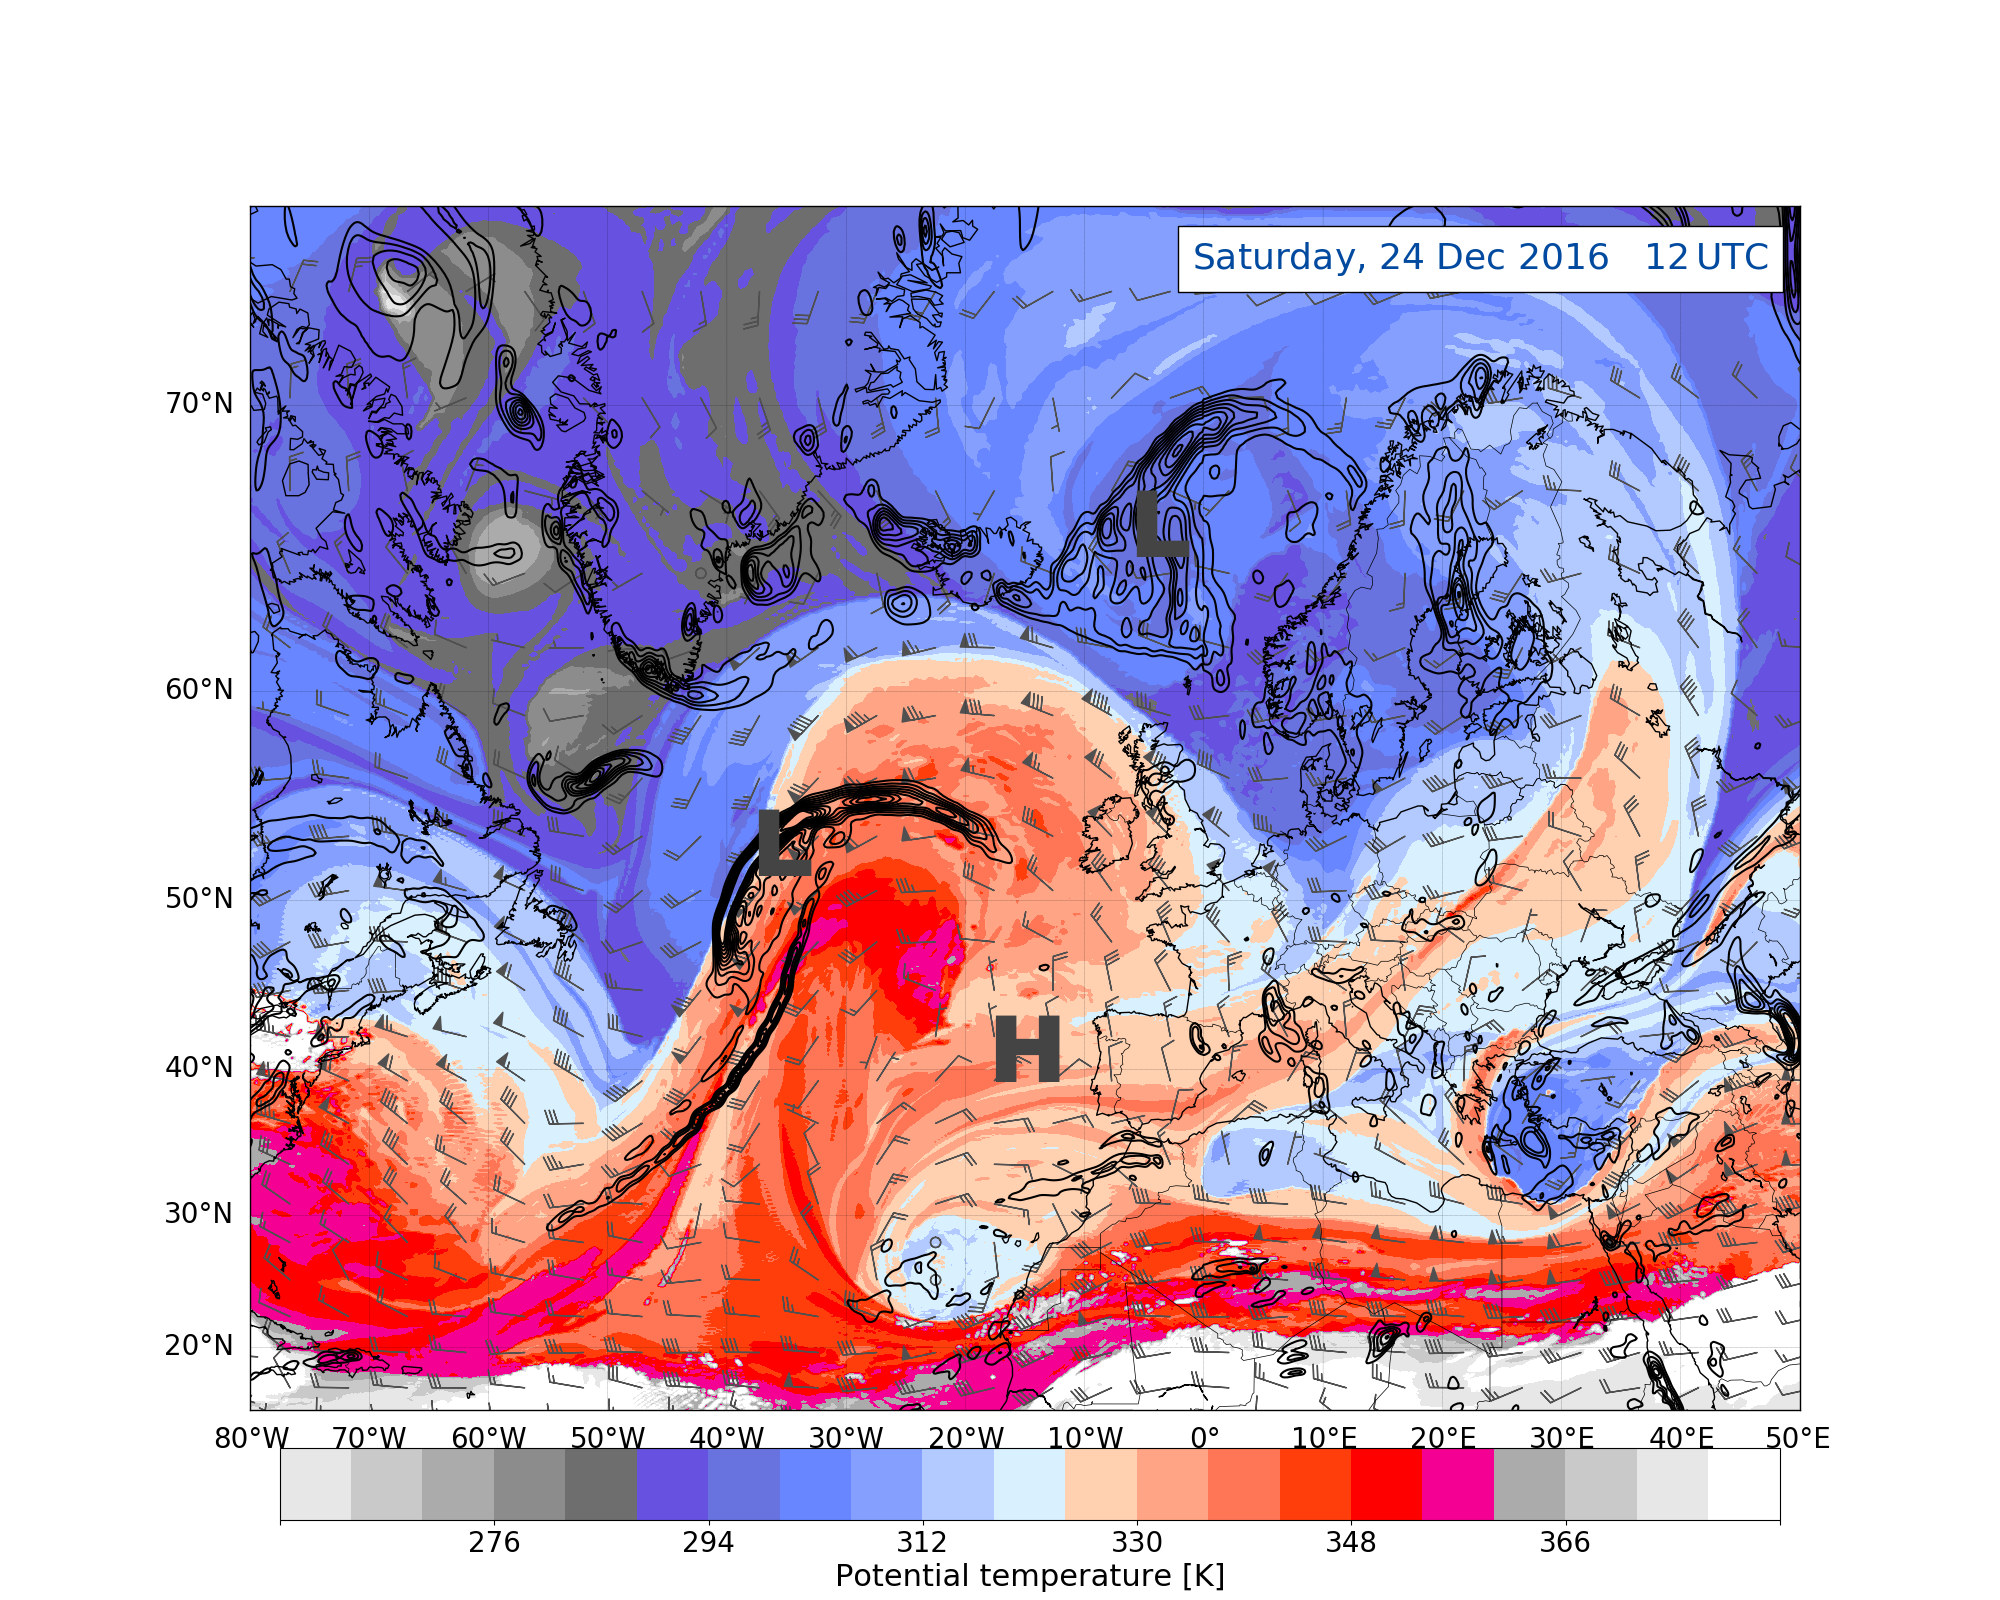
\includegraphics[trim={4.2cm 0cm 4.3cm 5.1cm},clip,
        width=\textwidth]{./fig_DynTropo/20161224_12_pres}
\end{minipage}\hfill
\begin{minipage}[b]{.4\textwidth}
	\captionof{subfigure}{Dynamic tropopause analysis map at \SI{2}{PVU}. Potential temperature [K] at the \SI{2}{PVU} surface, shaded according to the colour bar. Total wind, barbs [\SI{}{\mPs}], and \SI{925}--\SI{850}{\hPa} layer-averaged surface relative vorticity (black contours, every \SI{.5e-4}{\per\second}).} \label{fig:DT24_pres}
\end{minipage}
%%%%%% 20/12 slp thickness
\noindent\begin{minipage}%[t][0.55\textheight]
[t]{.59\textwidth}
  	\centering
  		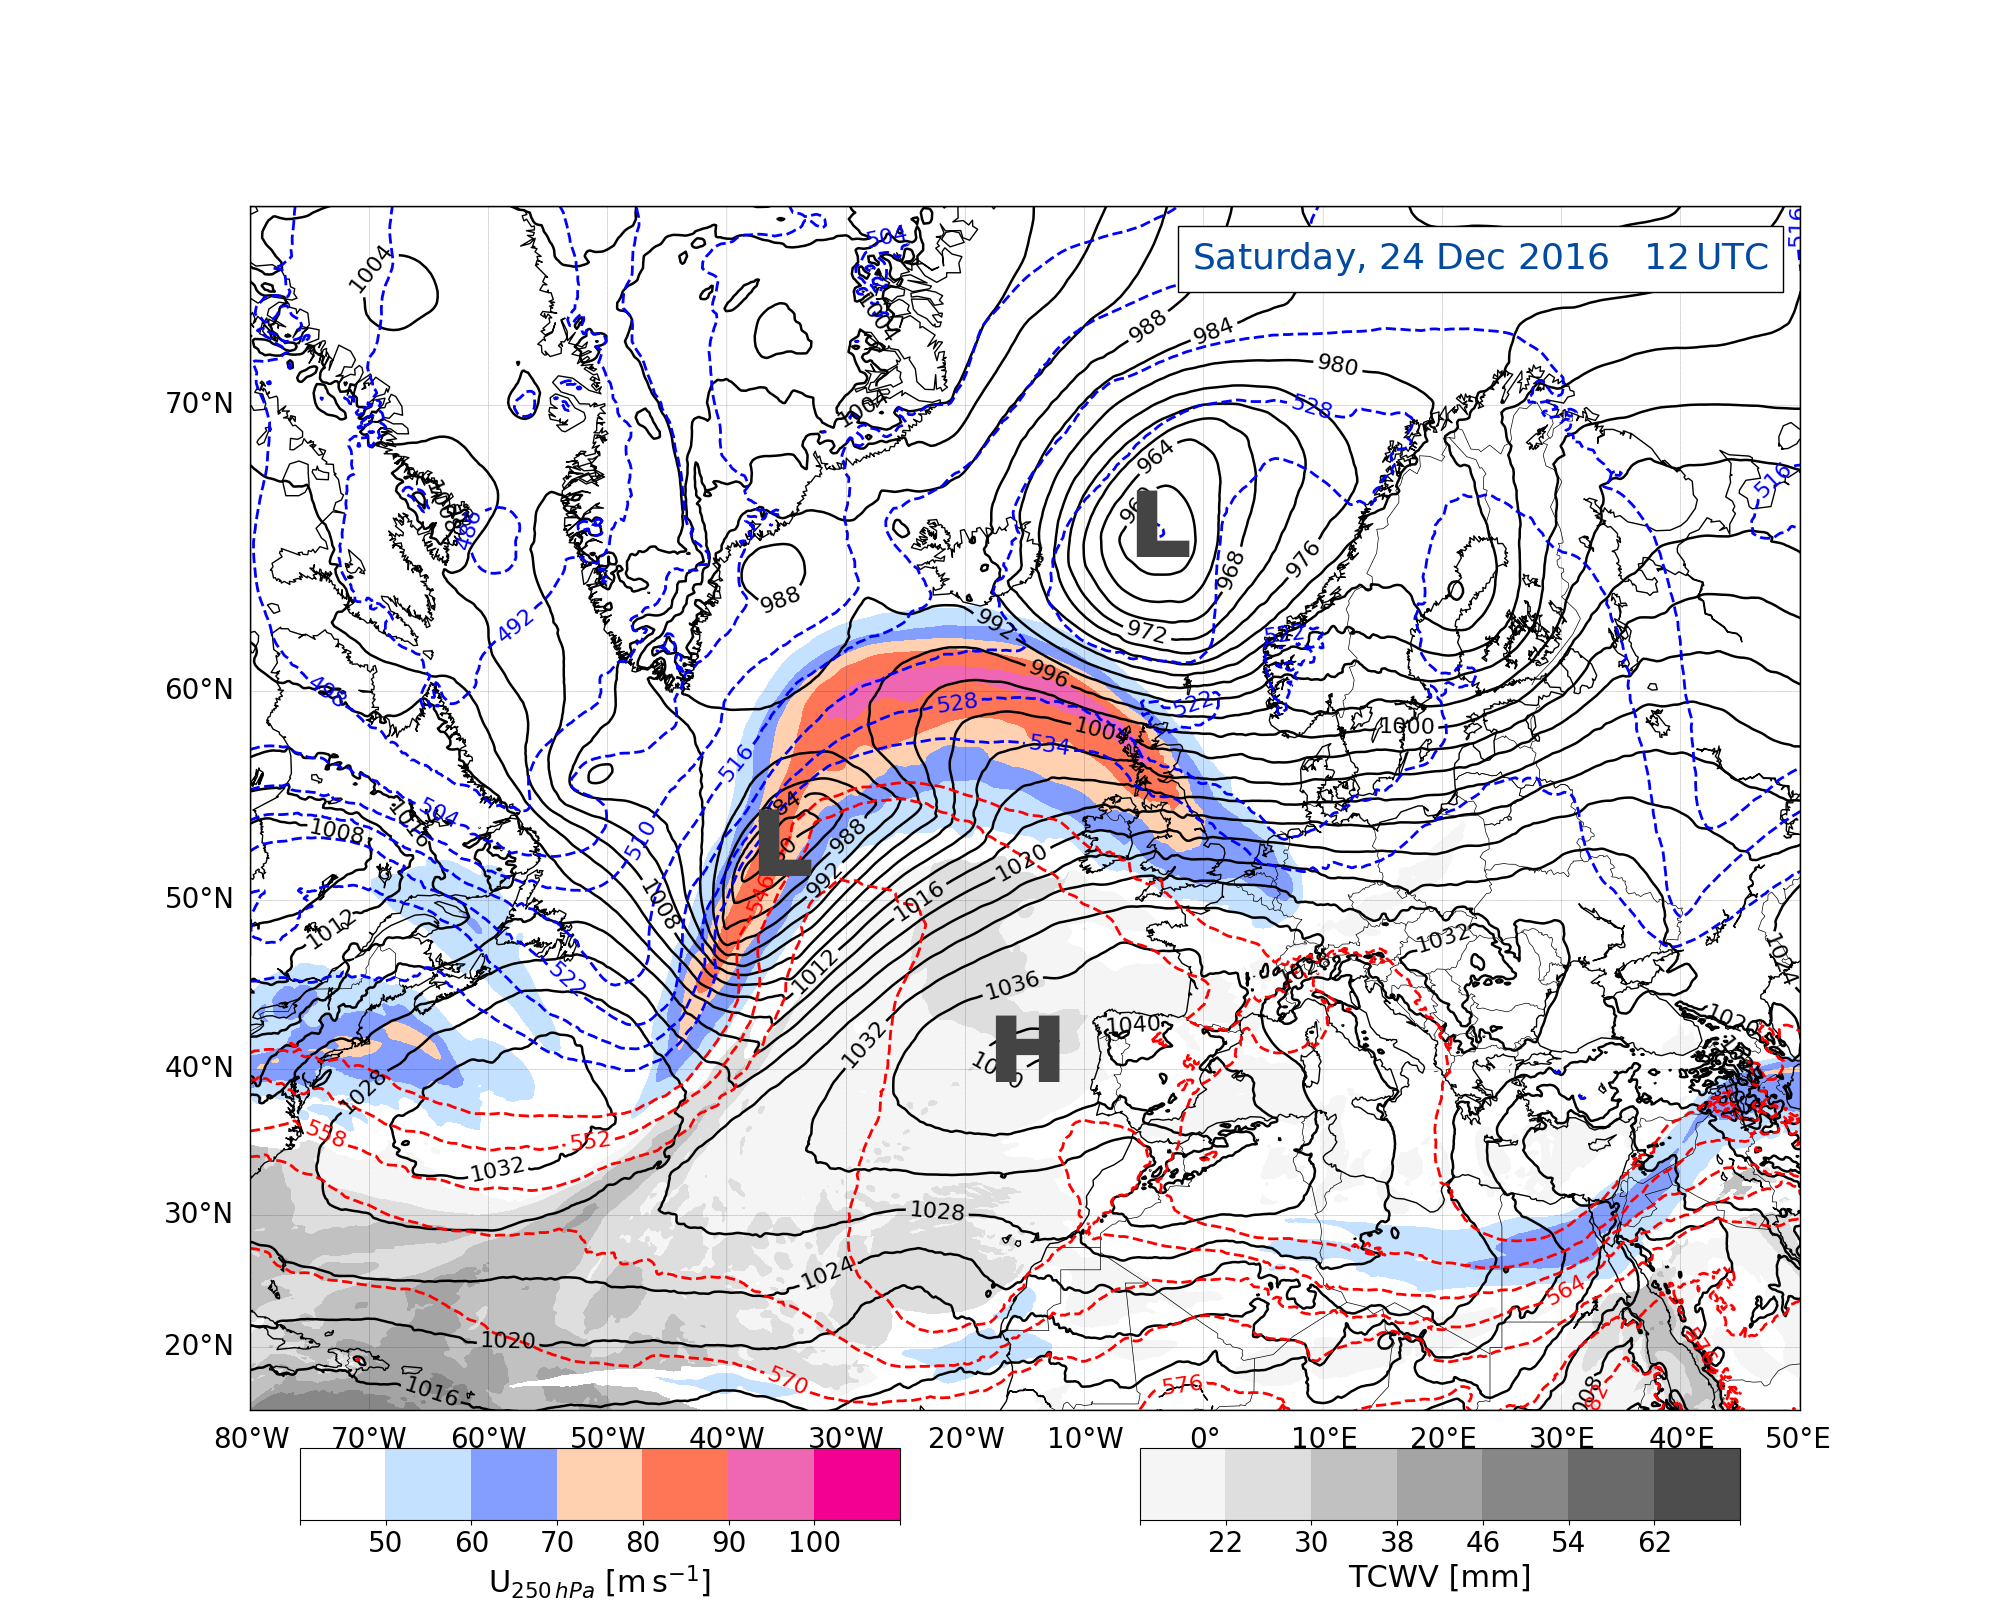
\includegraphics[trim={4.2cm 0cm 4.3cm 5.1cm},clip,
         width=\textwidth]{./fig_Geopot_Jet/20161224_12_pres}
\end{minipage}\hfill
\begin{minipage}[b]{.4\textwidth}
	\captionof{subfigure}{Jet, thickness, mean sea level pressure, and total precipitable water synoptic analysis. \SI{250}{\hPa} wind speed, shaded according to the colour bar, [\SI{}{\mPs}]. \SI{1000}-\SI{500}{\hPa} thickness, dashed contours every \SI{6}{\deca\meter}, MSLP, black contours every \SI{4}{\hPa}, total column water vapour [\SI{}{\mm}], shaded according the grey scale.} \label{fig:GP24_pres}
\end{minipage}
%%%%%% 20/12 IVT
\noindent\begin{minipage}%[t][0.55\textheight]
[t]{.59\textwidth}
  	\centering
  		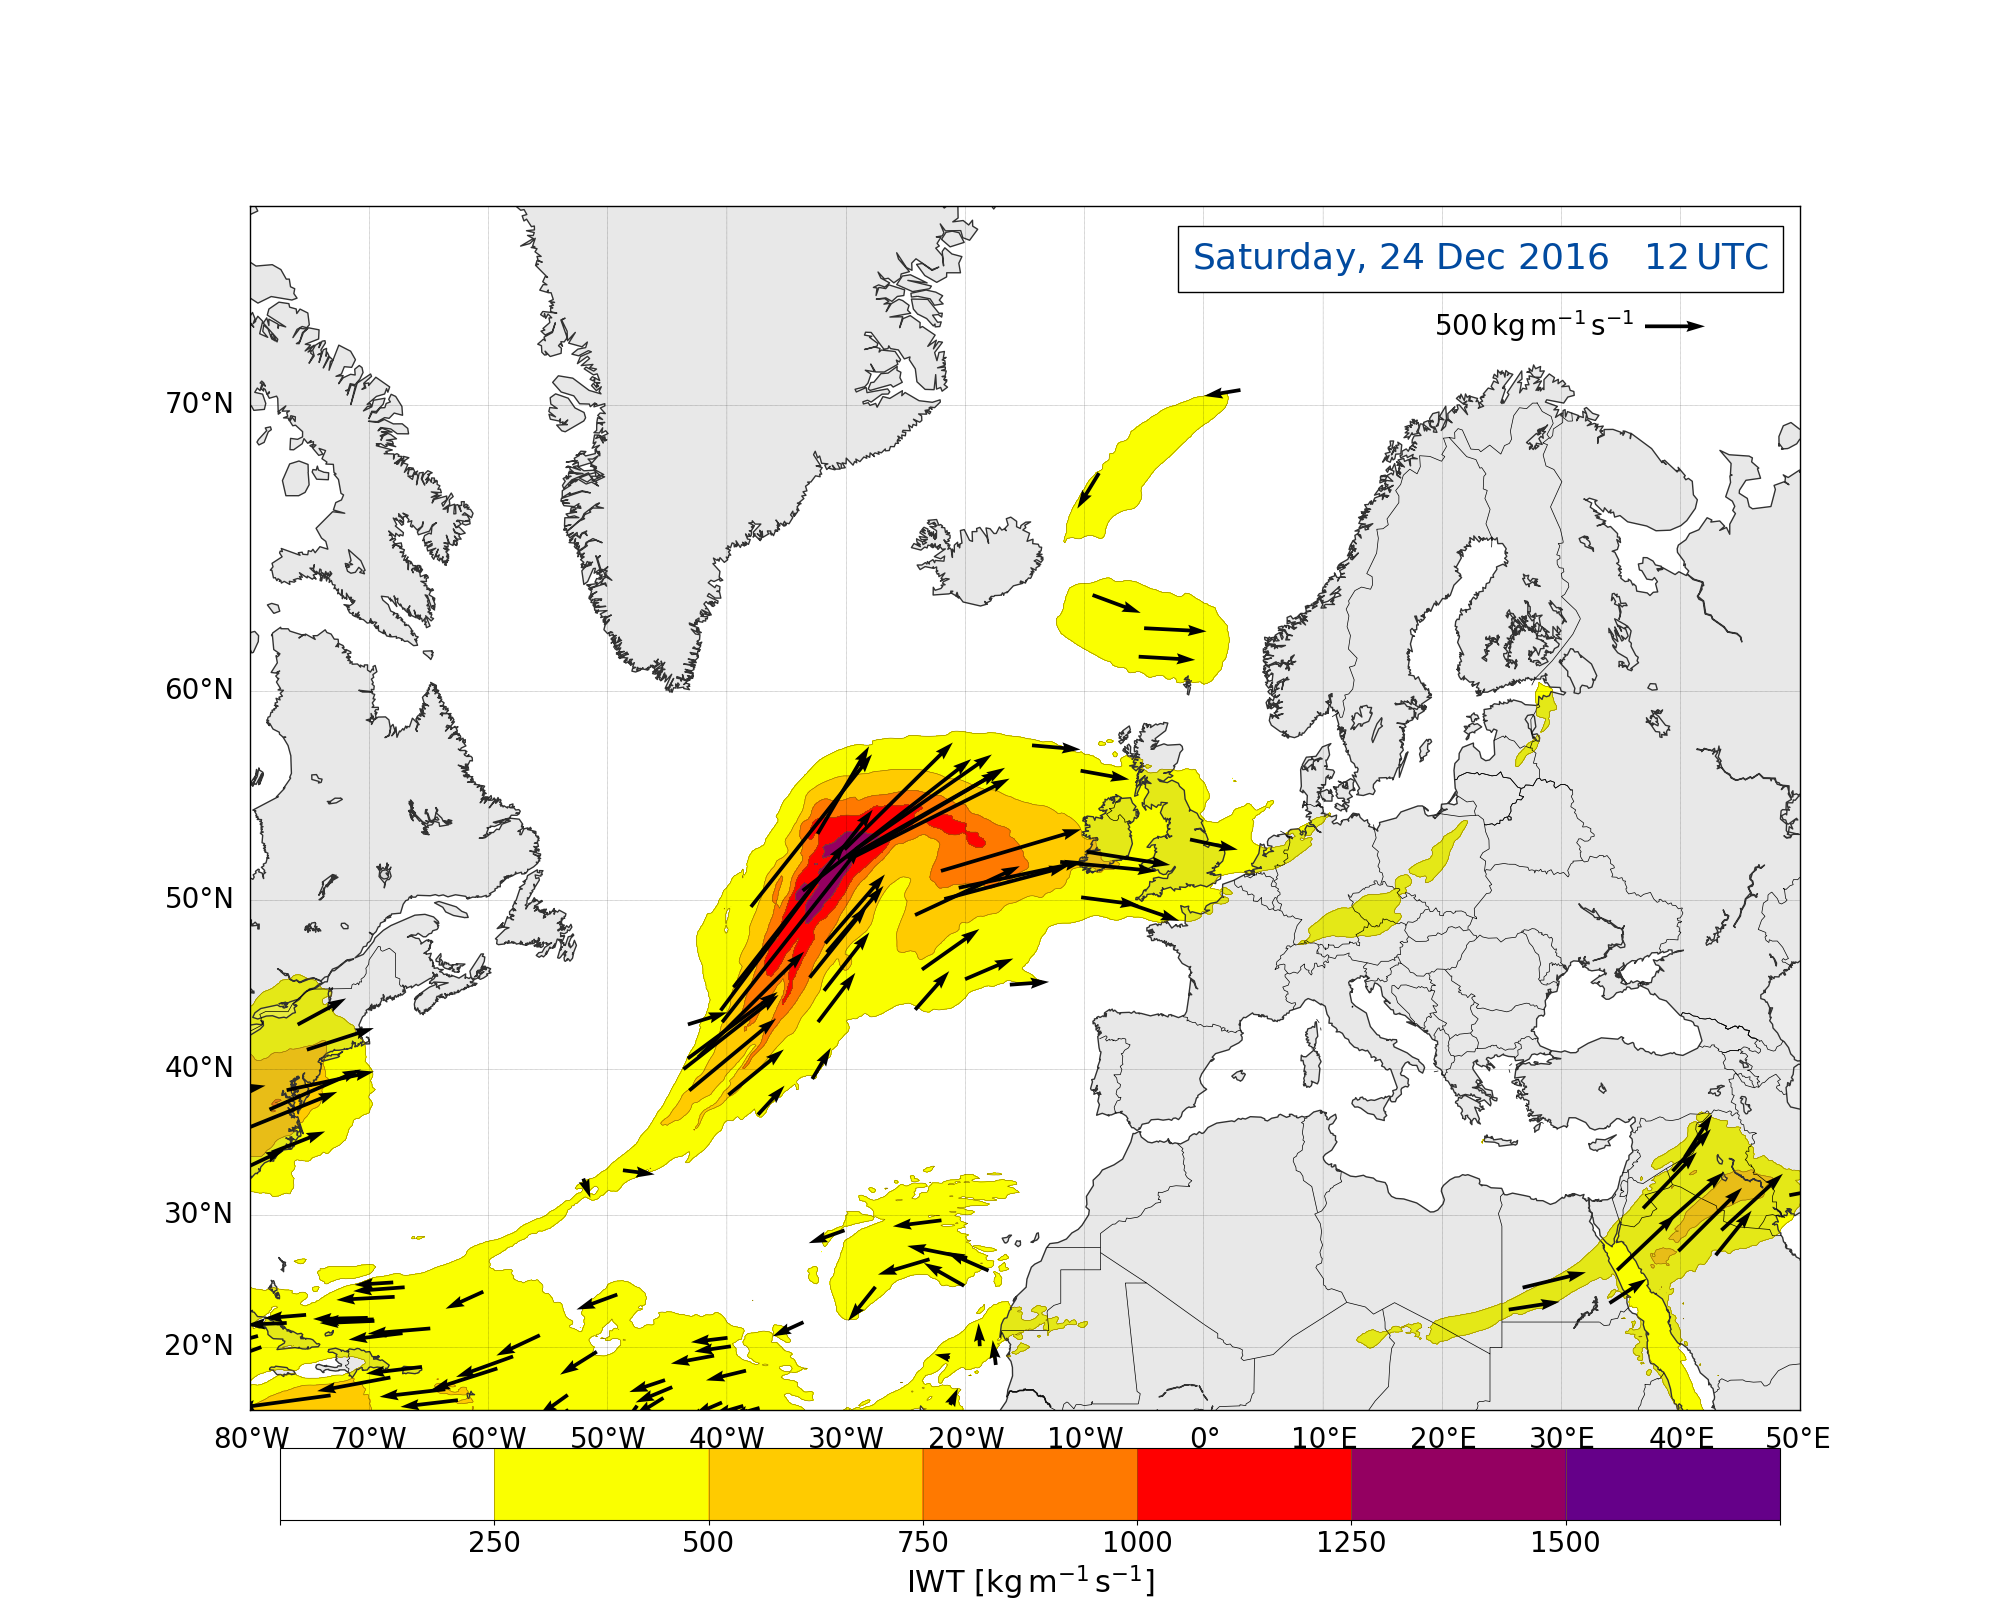
\includegraphics[trim={4.2cm 0cm 4.3cm 5.1cm},clip,
         width=\textwidth]{./fig_Atm_Riv/20161224_12}
\end{minipage}\hfill
\begin{minipage}[b]{.4\textwidth}
	\captionof{subfigure}{Integrated vapour transport analysis map. Integrated vapour transport, shaded according to the colour bar [\SI{}{\IVT}]. Vectors, indicating the direction and magnitude of the IVT. } \label{fig:AR24_pres}
\end{minipage}
\captionof{figure}{ECMWF analysis on \SI{24}{\dec} at \SI{12}{\UTC}. L and H indicating the surface low and high pressure, respectively.}\label{fig:24_12_pres}